\glsresetall

\section{Software Defined Networks History}
Traditionally, networking  relied and evolved over a non-transparent distributed model for the deployment of protocols and configuration of devices that resulted in: complex protocols and intrinsically difficult configuration of network devices. 
\gls{sdn} presents a new way of thinking in networking, shifting the complexity of protocols and management functions from  the  networks devices to a general purpose logically centralized service. 
The motivation behind this decoupling is the following: if the distributed network state can be collected and presented to a logically centralized service then it is simpler  both to specify network level objectives as well as to translate these objectives into the appropriate configuration of network devices. 
These planes, when loosely coupled, can simplify the development of protocols and the management of network infrastructures. 
%\gls{sdn} breaks this complex model through the physical detachment of the control and data planes.  

This section outlines the major contributions in the \gls{sdn} research field.   
In order to understand how \gls{sdn} works today it is fundamental to understand how they came to be. 
Understanding the biggest contributions in the \gls{sdn} research field allows us to draw a better picture of its skeleton, benefits and drawbacks. 
To do so, our  historical perspective hand-picks works that have structured the current \gls{sdn} architecture. 
%Our historical perspective hand-picks works that either have distributed control planes (thus being relevant for our work) or contribute with fundamental concepts to the current \gls{sdn} architecture. 
\gls{sdn} contributions can be decomposed  in three phases: the introduction of programmable network hardware; the control and data plane separation; and, finally the de facto standardization of the data plane interface~\cite{feamster2013road}. 
We only cover the last two since they are the ones that have a bigger impact in our work. 
For an overview of all the existing work we redirect the reader to the survey by Feamster~\etal~\cite{feamster2013road}. 


% In \gls{rcp} decoupled the control plane from the data plane just to solve routing problems. Then the 4D architecture formalizes a general architecture whereby all the control functionality resides outside the data plane.  This architecture was later adopted by the Ethane system. Finally the standardization of a data plane protocol and the introduction of a general, developer friendly, Network Operating System allowed \gls{sdn} to pull up the ladder. 


\subsection{RCP}
\glsreset{rcp}

In 2004 Feamster~\etal\ proposed the \gls{rcp} architecture to solve scalability and/or correctness problems in the \gls{ibgp} protocol --- 
a crucial component of the Internet operation used between routers inside an \gls{as}\footnote{A collection of \gls{ip} routing devices under the control of one or more network operators.} to distribute external routing information~\cite{Feamster:2004tg}. 
%Thus, it is an crucial component for the Internet operation.
A year later Caesar~\etal\ describes and evaluates a functional \gls{rcp} system~\cite{Caesar:2005ws}. 
%The \gls{rcp} system is one of the first to decouple the control plane from the data plane. 

With standard \gls{ibgp}, we must choose between scalability or correctness. 
%Both works identify scalability or correctness as the major problems in \gls{ibgp} deployments.
%On one hand, in a full mesh configuration, each router maintains  $O(n^2)$ (for $n$ routers) connections and associated state. 
On one hand, a full mesh configuration is correct, but requires a connection between any two routers, which significantly hinders the scalability of the system. 
On the other hand, the route reflection technique used to mitigate this scalability problem imposes a hierarchic structure between routers that narrows their knowledge of the routing state, which can cause problems such as route oscillations, and persistent forwarding loops. 
In contrast, routers in the \gls{rcp} architecture, send the routing information to a server that is responsible for routing decisions. 
As so, this server is able to maintain the global routing state in spite of operating with only one connection per router.
This architecture is able to scale better than the previous due to the lower number of connections, and it is correct given that the server has a complete view of the routing information.  

We note that the \gls{rcp} architecture is an \gls{sdn} whereby the routing state and logic are decoupled from routers (the data plane) and shifted to a server (the control plane). 
This was only possible owning to the fact that routers expose a well-defined interface for the dynamic configuration of the routing tables (the \gls{ibgp} protocol itself). 
As a result, the data plane configuration is defined in software by a decoupled server that has access to the global network view (the routing state). 
This is the definition of \gls{sdn}!

Caesar and colleagues advocate the distribution of the \gls{rcp} architecture in order to avoid a single point a failure and to amplify  the scaling ability. 
In this composition, each router connects to more than one \gls{rcp} server that can assign routes to any router under their command.
Interestingly, and in opposition to natural reasoning, the paper shows that \gls{rcp} does not requires a strong consistency protocol between servers in order to guarantee that the routes assigned by two different servers do not conflict (e.g., cause a loop) but, as laid out by the authors, this  observation relies on weak assumptions. 
%Interestingly, and in opposition to natural reasoning, the paper shows that it is not possible for two \gls{rcp} server to install conflicting rules in the same router even without the use of a consistent and/or coordination protocol between the servers (e.g., the consensus protocol described in section~\ref{sec:related:cons-data-stor}). 
First, it assumes a stable time period of the routing protocols whereby each server has a complete view of the routing state. 
Therefore, under transient periods of the routing updates the \gls{rcp} replicas might install conflicting rules in the routers. 
We add that the assumption also assures that all replicas see the same state (a property of strong consistency replicated systems). 
Second, the lack of a consistency protocol affects the liveness of the system because the servers might not assign routes to routers in order to avoid conflicts. 

\subsection{4D}
In 2005 Greenberg~\etal\ published a seminal paper proposing a clean slate network architecture, named 4D,  to address the (arguably) root problem of existent networks: the complexity that derives from twisting the control and data plane on the network elements. 
In this work the authors' argue that under this condition the management of networks is achievable only through ad-hoc manual intervention (which is error-prone); the specification of network level goals is difficult since the control functions do not work in concert; and the development of control functionalities is complex due to the distributed nature and scale of the data plane. 

The 4D architecture builds on 3 principles: specification of global network level goals (e.g., routing, security policy),  centralization of the network state \mbox{(e.g.,\ topology, link state),} and run-time configuration  of the network elements. 
With those principles one should be able to: shield configuration from the hazard of low level and protocol-specific commands distributed across devices, develop dynamic algorithms based on centralized network state\footnote{The reader familiar with networks protocols will  understand that this allows to use Dijktra instead of Bellman-Ford.}, and  to configure, in run-time, the network devices.  
To achieve this goals the authors' propose a network architecture structured in 4 layers (hence the name): the \textbf{data} plane to forward packets; the \textbf{discovery} plane to collect information from the data plane; the \textbf{dissemination}  plane to configure the data plane; and the \textbf{decision} plane to translate network goals and state into the configuration of the data plane. 
%However, 4D isolates functions in the dissemination and discovery plane that mingled together in current \glsplural{sdn} architectures. 

When compared to the \gls{rcp} architecture, 4D exposes the same patterns of decoupled planes, centralized network state, programmable devices, and so on and so forth... 
However, while \gls{rcp} only separates routing from routers, the 4D architecture envisions an extreme design whereby all control functionality is separated from the network devices. From the 4D perspective, devices should only be responsible for forwarding packets (that is it). Moreover, the authors' argue that it should be possible to leverage the existent forwarding mechanisms (e.g., forwarding tables, packet filters and packet scheduling) as a unified resource at the service of high-level network goals  (e.g., ``keep all links below 70\% utilization, even under single-link failures'').
Even if at the time this work ``generated both broad consensus and wide disagreement from the reviewers'', the current \gls{sdn} hype and existent work has been able to confirm much of the previsions and reasoning of their authors. 
In fact, the current \gls{sdn} architecture is very similar to 4D albeit the practical mingle of the discovery and dissemination plane in a single protocol (see section~\ref{sec:realted:softw-defin-netw}). Being so, \gls{sdn} owes much to this work, which has set a groundbreaking discussion and conceptual design that led to the development of real-world systems such as the one we present in the following section.  

\subsection{Ethane}
%While the 4D architecture was merely a conceptual ``vision'', several implementations followed it. 
In 2007  Casado~\etal\ presents a network architecture for the enterprise with emphasis in security~\cite{Casado:2007kb}. 
This architecture, named Ethane, follows the 4D footprints and identifies the same problems in the traditional network management domain. Namely, the configuration errors caused by distributed configuration and lack of cooperating control functions. 
To address those issues they introduce the controller as a logically centralized server in charge of all network devices.
By maintaining a global network view that includes topology and  bindings between users, host machines and addresses, the controller is able to play the interposition role between any communication occurring in the network. As such, it can ensure that a network policy is correctly respected. 


In Ethane network devices (switches) do not perform regular operations (e.g., learn address, packet filtering, routing protocols, etc.,).
Instead, they are limited  to flow-based forwarding with the help of a local flow table that is maintained by the controller. A flow broadly equivalent to a single host-to-host network interaction (e.g., all the \gls{ip} traffic destined to a host or  all the \gls{http} between two particular hosts). 
Every packet that fails to match with any of the rules available in the flow table is redirected to the controller. Then the controller takes the packet information, current network state and security policy and decides on a forwarding policy. Commonly the controller will either drop the packet or decide on a path and install rules in the switches such that  not only the packet but also packets that will follow it (i.e., a flow) find a match in the flow table thus avoiding being redirected to the controller. 


Arguably, the most significant contribution of Ethane came from the results obtained with the deployment in a particular campus network with approximately 300 hosts. 
According to the reported results, the authors estimate that a single desktop computer could handle a network with over 20k hosts.  
This is interesting since at the time,  one of the biggest objections to decoupled architectures was the scalability and resilience properties. 
Consequently  in the paper we also see a significant discussion regarding the resilience of Ethane. 

The authors present different distribution modes to achieve resilience. 
In the primary-backup mode  there is one active controller while others standby to take over its place in the event of failure. 
In this mode the standby controllers can keep slow-changing state (such as configuration and user registration) consistently while the binding information that associates network devices to users is kept under eventual consistency semantic. 
The only problem identified in the paper with this mode is that in the event of failures some users may need to re-authenticate. 
In the active mode, two or more controllers take over the network while switches distribute their requests across the existent controllers.  
Under this mode, the authors argue that  the use of eventually consistency semantics for replication is sufficient in most implementations. To  sustain it is observed that the use of consistency aware data structures such as \gls{crdt}\footnote{A \gls{crdt} is an special data structure that is used to avoid conflicts or loss of information in eventual consistent replication of data.} or simple partitioning schemes (e.g., separate \gls{ip} address space across controllers for \gls{dhcp} allocation) can be sufficient for avoiding inconsistency problems. 
Albeit arguing for eventual consistency they do state that there a need for further study and stronger consistency guarantees such as the \gls{smr} used by in our distributed control plane. 

We do not disagree but we also do not agree. 
We believe that in a sensible deployment where the security policy must be strictly respected in every host-to-host communication, it is crucial that the distribution of the control plane is built on top of resilient and coherent distribution models. 
However due to the asynchronous nature of a network (e.g., as soon as you install a rule in a switch, the network policy or topology may already have changed) we may need more than a strong consistency semantics for the control plane. In fact, we may need to expand the strong consistency semantics to the data plane (as covered in section~\ref{sec:related:consistent-data-plane}). 
Finally, as explained in section~\ref{sec:related:cons-data-stor} the use of eventually consistent data stores requires extra work and care from the developer that we do not believe to justifiable in all cases. 

To summarize, Ethane was one of the first examples  of a functional \gls{sdn} architecture capable of fully operating with all the control logic separated from the network devices that were reduced to simple forwarding equipment that was configured in run-time by the controller with the help of a logically centralized network state.  

\subsection{OpenFlow}
\label{sec:related:openflow}
In 2008, McKeown~\etal\ introduced the \gls{of} protocol that would soon become the defacto  standard to program network devices thus ``enabling'' the broad adoption of \gls{sdn} architectures in the years to come~\cite{McKeown:2008dn}. 
OpenFlow  enables a standard interface to program devices that were previously closed by nature. 
A common analogy is to compare network devices to processors and \gls{of} to an instruction set that exposes the underlying functional through a well-defined interface. 
In \gls{of}, as in Ethane, network devices are limited to flow-based forwarding only. 
A flow table resides in the network device and is composed of tuples $\langle match,action \rangle$. 
The $match$ entry allows the device to match arriving packets, while  $action$ specifies the forwarding behavior. 
Switches can match packets against standard fields in Ethernet, IP, and transport headers and follow actions that can range from drop, forward to single port(s), or forward to the controller. 
The controller can install and manipulate this table as he sees fit. 
We cover \gls{of} in more detail later (see section~\ref{sec:related:openflow-spec}). 

OpenFlow rises from the success of previous systems like Ethane.
In fact, McKeown and colleagues do not introduce any groundbreaking novelty with respect to Ethane but rather generalize a technology already seen possible in Ethane switches. 
Furthermore, the paper can be seen as a ``call to arms'' or an appeal to two different communities: the industry community to adopt the protocol in their equipment; and the academic community to push for innovation even outside the \gls{sdn} context. 
The protocol  was quickly adopted for three reasons. 
First, it lowers the innovation barrier by ``opening''  the existent networks (and correspondent devices) to the deployment of new protocols that could even run isolated from production traffic. 
Second, it also lowers the innovation barrier for the development of \gls{sdn} architectures. 
Third, the \gls{of} interface contract only requires capabilities that were already present in the hardware thus network devices could support it with a simple firmware upgrade. 

In summary,  OpenFlow generalizes the switches that we already seen in Ethane. 
As ``asked for'' in the paper, several of the  network manufacturers have included the \gls{of} technology which has allowed the development and research of numerous \gls{sdn} based network advancements. 

\subsection{Network Operating System}
\glsresetall
\label{sec:related:netw-oper-syst}
With the adoption of the \gls{of} protocol \gls{sdn} a gained significant momentum. 
However, the existent work up to this point focus in monolithic control plane to satisfy specific network goals (e.g., routing in the Routing Control Platform, security in Ethane). 
While \gls{of} generalizes the data plane interface there is  the need for an abstract and general control plane that consolidates the network control functions. 

In the context of SDN it was, to our knowledge, introduced by Gude et al. \cite{Gude:2008jd} and Cai et al. \cite{Z.-Cai:2008fk}.
Both works decompose the control plane in two layers: Management and Control. 
In the Management layer resides the application logic divided into applications according to their different network goals (e.g.,routing, firewall, load balancing). 
Supporting this logic is the Control layer that provides a Network Operating System whereby the Management applications reside. 
This Operating System provides the common functionality that out to be shared between all applications such as network device communication (e.g., through OpenFlow), state management and application coordination. 
Those tasks are roughly comparable to a regular Operating System (i.e., device drivers, shared memory and scheduling). 


The role of the \gls{nos} is enable the development of a broad spectrum of network applications that can ultimately cooperate and share information. This ability is provided by a programming interface and should allow to control and observe the state of the network. 
In section~\ref{sec:related:phys-centr-contr} we explore how the current state of the art manages this. 
Interestingly, until this day the architecture of the \gls{nos} has not changed drastically, and both these papers had a deep impact on the existent open source controllers that we see today. 
%%%%%%%%%%%%%%%%%%%%%%%%%%%%%%%%%%%%%%%%%%%%%%%%%%
\glsresetall

\section{Software Defined Networks Fundamentals}
\glsresetall
\label{sec:realted:softw-defin-netw}


In March 2011, the Open Network Foundation (ONF) was created with the participation and support from several industry partners \cite{onf}. 
ONF  is a ``non-profit consortium dedicated to the transformation of networking through the development and standardization of a unique architecture called Software-Defined Networking (SDN)''. 
They have done so, by releasing a white-paper defining the design principles for a SDN architecture and the advantages of it \cite{ONF:2012ui}. 
They are also responsible for the standardization process of the OpenFlow protocol.

The \gls{sdn} architecture is not a standard but rather an architectural approach to networking. 
It should be clear, by now, that \glsplural{sdn} are based on three essential design principles: decoupling of the control plane from the data plane, logically centralized network view, and programmable remote access to network devices. 

So far, the \gls{sdn}  architecture has not converged on well-defined interfaces that we could use as reference to define its meta-architecture. 
In fact, it might be the case that it will never will. 
Nonetheless, there are common elements throughout most of the existent \gls{sdn} literature. 
Consequently, this section defines a common language  used throughout this document to refer to different \gls{sdn} components.
This includes a definition of a meta-architecture for the \gls{sdn} stack (section \ref{sec:related:sdn-architecture} and an overview of the most common data plane interface: OpenFlow (section \ref{sec:related:openflow-spec}). 
This section can (and should) be used as reference throughout the text. 

\subsection{SDN Architecture}
\label{sec:related:sdn-architecture}
The common \gls{sdn} architecture is a three-layer stack shown in Fig.~\ref{fig:related:sdn-stack}. 
% \begin{itemize}
% \item Context. 
% \item This architecture is not written in stone. Multiple variations and complete extremes are possible. 
% \end{itemize}

\begin{figure}
  \centering
    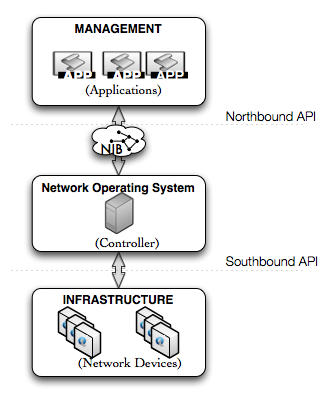
\includegraphics[width=\textwidth]{pic/related/sdn-stack}
  \caption{SDN Architecture}
  \label{fig:related:sdn-stack}
\end{figure}

%The image is misleading in severals ways (for the sake of simplicity). First, the applications (APP) do not necessarily reside outside the control plane. 
%They can be located in memory with the controller process. 
%Second, the network state also does not necessarily reside outside the control plane in a data store. 
%It could also be located in memory, or in extreme do not even exists (e.g., each application maintains its relevant state). 

The network logic operates in the \textbf{Management} plane. 
This plane defines the global network level objectives in the form of one or more (possibly) cooperative applications. 
From a conceptual point of view, these applications interact with the controller through the \emph{North} \gls{api}. 
% In practice this is not always true (explained further along the text). 
A possible implementation of this interface is a \gls{rest}  web service implemented in the controller\footnote{A web \gls{api} based on \gls{http} protocol.}~\cite{fielding2002principled} that allows remote applications to read and modify the network state and configuration.  
It is also possible that controllers allow applications to subscribe (to be process) to network events through this \gls{api}. 
This is typically applicable to in-memory applications but does need to be the case. 
For this reason the image also shows that the controller invokes operations on  the Management plane through the \emph{North} \gls{api}. 
All the control planes referenced in this document allow this behavior for in-memory applications. 
In fact, as we shall see, the event-oriented programming model is present throughout all the \gls{sdn} stack components  being that  \gls{sdn} is event oriented from the get go, as network events  such as  topology changes and forwarding requests, are asynchronous in nature. 

In the \textbf{Control} plane resides the core logic that glues the stack together. 
This component has three major responsibilities. 
First, it is responsible for orchestrating the multiple applications available.
This implies setting up the remote \textbf{North} \gls{api} (e.g., \gls{rest} web server) and maintaining in memory applications that cooperatively manage the network. 
Second, the controller  defines how the \emph{Network State} is shared between  applications. 
In the event that the control plane is distributed, then the controller also defines how the state is shared between controllers. 
%It may also define how this state is shared between controller if the control plane out to be distributed (explained further along in the text). 
%Applications that maintain network state such as topology are commonly provided by  the controller, and usually operate in-memory. 
%usmaintaing a platform where the in memory applications reside that cooperatively builds and maintain the \emph{Network State} with all the relevant information for the control platform in place (e.g., switch and link state,  topology, firewall rules, etc.,).  
Third, it is also in charge of the data plane communication, through the \emph{South} \gls{api}  that enables data plane configuration (e.g., push/pull state from switches). 
Again, the \emph{South}  \gls{api} can be event-oriented whereby events are commonly topology information (i.e., link up, link down) or forwarding requests (e.g., flow tables misses in \gls{of}). 

Finally, the network devices responsible for packet forwarding reside in the  \textbf{Data} plane. 
Any device can be used (wireless access point, Ethernet Switch, router), as long as it implements the \emph{North} \gls{api}\footnote{In practice a mixture of both north enabled  enabled devices and normal devices is possible. Those are known as hybrid networks by the \gls{sdn} community.}.
We commonly refer to these elements as switches regardless  of the functions that they perform in a standard mode (without the intervention of a controller). 

There must be connectivity between the Control and the Data plane.
This connectivity can be  \textbf{in-bound} or \textbf{out-bound}. 
In the in-bound case, the connectivity takes place over the network used for data forwarding while in the out-bound case a different and isolated network is used. 
Connectivity between these two layers require manual configuration of the network devices. 

The \emph{West}/\emph{East}  \gls{api} is  the same and exists only when  distributed control is employed (see Section~\ref{sec:related:distr-contr}). 
Then, the controller uses this \gls{api}  for state distribution and controller-to-controller communication. 
It has two flows of communication for functions performed by the controller on another controller instance (e.g., push state, read state, install rules in another switch, etc.,) or in event-oriented  implementations to receive events from other controllers (e.g., state has changed, new data plane event from a switch). 

Finally, we note that \glsplural{sdn} can operate in two different models. 
In the  \textbf{Reactive} model a switch that does not known how to forward a packet can request the controller to chip in. 
The controller can then take action (e.g., forward, drop, log)  and inform the switch. 
Typically (as shown in Fig.~\ref{fig:related:reactive}) the controller updates the switch with rules for both the packet and subsequent packets that will follow it.  
In contrast, in a \textbf{Proactive} model the switch does not contact the controller with  forwarding requests. 
Instead, the switch is configured according to the management networks objectives. 
Whenever this objectives changes or the network state changes (e.g., link goes down) then the control plane updates the configuration of the switches. 
We note however that the current \gls{sdn} technology is pliable enough to have both models. 
One can even choose between the two models for different types of traffic, or different periods of time in the same \gls{sdn} deployment. 

\subsection{OpenFlow}
\label{sec:related:openflow-spec}
\glsreset{of}
%Missing things to talk about:
% \begin{itemize}
% \item FLOW REMOVED (evaluation section, maybe we can remove it). 
% \item FLOW MOD  (evaluation section, maybe we can remove it). 
%\item it is event-driven, the switch does not need a reply
% \end{itemize}
\gls{of} is the most common implementation of the \emph{South} \gls{api} shown in Fig.~\ref{fig:related:sdn-stack} which consequently has  
somewhat defined the current panorama of \gls{sdn} architectures. 
Thus, in order to make this document self-contained we feel that we should clarify some technical aspects of the \gls{of}  protocol. 
%This section will briefly resume (and simplify) the most important characteristics of the protocol that should be used as reference for the remaining document. We note that the relevance of this protocol has already been covered in section~\ref{sec:related:openflow}.  

\begin{figure}
  \centering
  \includegraphics[width=\textwidth]{pic/related/openflow}
  \caption[Flow Request ]{Commonly, in an reactive model, the first packet of an flow for which there is no match is forwarded to the controller which evaluates it and decides the appropriate action. Normally it modifies the switch flow table such that the packets that follow do not have to go to the controller. }
  \label{fig:related:reactive}
\end{figure}

\begin{table}[ht]
  \centering
  \begin{tabular}[ht]{lll}
    Match Fields &  Instructions & Timeouts \\ \toprule 
    source MAC = 10:20:. \emph{AND}  protocol = ICMP  & port 2,3 & 5,10 ms \\ 
    source IP = 10.0.0.0/24  & port 1 &  0/0 \\
    source IP = 10.0.0.0/24 \emph{AND} protocol = TCP & controller & 0/0 \\ 
    any & controller & 0/0 \\ \bottomrule 
  \end{tabular}
  \caption[Openflow Flow Table]{Simplified representation of a flow table in OpenFlow switches.}
  \label{tab:related:openflow-flows}
\end{table}

Table~\ref{tab:related:openflow-flows} shows a representation of an \gls{of} table present in the switch.
This table is used by the controller to define the forwarding rules for each packet in the network that passes through the switch. 
%The switch uses the match fields to find the forwarding instructions for any incoming packet.
As opposed to common devices, which are restricted to a small set of network packet headers (e.g., \gls{mac} for switches, \gls{ip} for routes), \gls{of} switches are able to match packets against 13 different headers (that can be combined with logical operators).
Furthermore, some headers such as the \gls{ip} and \gls{mac}
 fields can be matched against  bitmasks which allows  a wide range of values for a single table entry. 
As an example, the table shows that the last two entries match against any host present in the $10.0.0.0/24$ network. 
Beyond headers, the switch can also match packets according to the port on which they arrive. 
We note that conflicting matches (i.e., a packet matches more than one entry in the table) are arbitrated by the priority associated with the rule (not show in the table). 

For each entry there is an associated instruction that the switch uses to forward the packet whenever it is able to find a match. 
Several instructions are available including: forward to port $x$, forward to controller, and drop the packet. 
As seen in the table, the instructions can be combined (the first entry forwards to two different ports). 


Each entry  is removed from the table once one of the two private timeouts expire. 
There is an hard timeout, which is never reseted,  and an  idle timeout that is reseted whenever an packet is matched against the entry. 
Both timeouts are used by the controller to recycle and control the entries in the switch table.
It is also possible that a rule is persistent (never expires). 
In this case the timeout will be set to 0. 


A \gls{of} switch table can be configured to forward non-matching packets to the controller (e.g.,  the last entry in the table).
In a  reactive model, the switch forwards the first packet of a flow to the controller. 
In this context flow is somewhat undefined but in essence it should represent a stream of one or more packets in an communication.
For example a flow could be all the packets exchanged between an \gls{http} client and server to download a web page, or it  all the \gls{icmp} packets exchanged between a pair of hosts. 

Fig.~\ref{fig:related:reactive} illustrates how the switch processes packets in the reactive mode. 
The first packet (1) for some ``flow'' (e.g., download of an web page)  reaches the switch but is redirected to the controller since there is no rule that matches it in  the switch table. 
We call this message (from the switch to the controller)  a flow request or \texttt{packet-in}. 
This request must contain (at least) the packet header from packet 1 that will be used by the controller to determine the reply. 
For this reason we usually abuse the language and say that a packet arrives the controller. 
For example, we might say an \gls{ip} packet arrives at the controller to refer to a flow request caused by an \gls{ip} packet. 
Getting back to our example, when the controller receives a flow request, he processes it  and then replies to the switch with instructions to process the packet. 
Additionally, the controller also configures the switch table such that  future packets in the flow are forwarded directly by the switch. 



%%%%%%%%%%%%%%%%%%%%%%%%%%%%%%%%%%%%%%%%%%%%%%%%%%
\glsresetall

\section{Physically Centralized Controllers}
\label{sec:related:phys-centr-contr}
\glsresetall

%%%%%%%%%%%%%%%%%%%%%%%%%%%%%%%%%%%%%%%%%%%%%%%%%%

In this section we present an overview of relevant centralized
controllers. Centralized controllers are, by our definition, control
planes that do not show any explicit support in the deployment of 
different controllers processes over onde or more servers. 
According to our general architecture (see section~\ref{sec:related:sdn-architecture}) the controller has no \emph{East}/\emph{West} \gls{api}. 


\begin{figure}
  \centering
\includegraphics[width=\textwidth]{pic/related/meta-controller-architecture}
  \caption[Controller Architecture]{The common (meta) controller architecture is event-driven. The data plane triggers events (e) that are dispatched by the controller to a pipeline of interested applications. }
\label{fig:related:meta-architecture}
\end{figure}

All the controllers in this section share the architectural composition shown in Fig.~\ref{fig:related:meta-architecture}.
In this architecture, the controller supports multiple applications that run in-memory (i.e., with the controller process) with the goal of processing events  triggered by the data plane (i.e., the switches). 
For each event $e$ (e.g., link up, new switch, flow request) the switch triggers an \gls{of} message to the controller. 
This, in turn, parses  the message to analyze its type and redirects it to the appropriate pipeline. 
A pipeline, is composed of several stages. 
In each stage a different application processes the event and chooses to pass it further along in the pipeline, or to abort the event processing. 
We note also that any (or all) of the applications could interact with the switches at any time. 
Finally we also notice that this architectures  show a tight-bound between the Management and Data plane interfaces (i.e., \emph{North} and \emph{South} \glsplural{api}) since the pipelines are dependant of \gls{of} events. 

This architecture has been concurrently introduced (see section~\ref{sec:related:netw-oper-syst}) by NOX (covered in section~\ref{sec:related:nox}) and Maestro (covered in section~\ref{sec:related:maestro}).  It was also adopted by Beacon (section~\ref{sec:related:beacon})  and later on Floodlight (section~\ref{sec:related:floodlight}). 
We have evaluated and studied all this controllers considering each one as the base for out distributed controller. 
We end up choosing Floodlight for this and we explain why in section~\ref{sec:related:controller-choice}. 

\subsection{NOX}
\label{sec:related:nox}

NOX\footnote{\url{http://www.noxrepo.org/}} was published and publicly released under
the \gls{gpl} in 2008 \cite{Gude:2008jd}. 
It was developed both in C++ and Python and enables a standard interface for the integration of  Management applications 
in the controller. 
Even though one of the main contributions of this paper is the introduction of the \gls{nos}  abstraction (see section~\ref{sec:related:netw-oper-syst}, NOX itself  is tightly bound to the \gls{of} \gls{api}. 

The NOX programming model is event-driven as shown in Fig.~\ref{fig:related:meta-architecture}.
Applications  register in a
priority based pipeline with event handlers associated to either OpenFlow  or application based events. 
The NOX core is equipped with applications that build a host and switch level topology in the network \emph{view}. 

In NOX applications control network objectives and also cooperate to define the current \emph{view} which is an essential component of the controller. 
The \emph{view} can contain the switch-level topology; the location of users, hosts, middleboxes and other network elements; and the services (e.g., \gls{http}) being offered. 

Interestingly, the authors' point out that this choice of granularity for state (the \emph{view}) is adequate for many network applications while changing slowly enough that it can be scalably  maintained. 
They also argue that the network \emph{view} can be distributed with standard replication techniques for resilience. 
In fact the \emph{view} is a set of indexed hash tables with support for local caching. 
In this regard this vision is very similar to ours but has not been effectively developed in their work. 

Initially, NOX was a single threaded application not focused on performance. 
However, from its publishing date several improvements have taken place \cite{Tootoonchian:2012uia,zen-doc-thesis} that have significantly improved NOX performance. 
Under the set of improvements we highlight the natural evolution to a multi-core aware application that statically distributes network requests to different threads. 

In the time of writing, NOX is publicly available but has ramified into two different applications: A C++ based controller available in Linux and a Python based controller (POX) available for several environments.

\subsection{Maestro}
\label{sec:related:maestro}


A network operating system has (at least) two functions: introduce a layer of abstraction between the network and the applications and control the interaction between applications. Maestro is the undergoing work of Zeng Cai covered in \cite{maestro} is focused in the second. In particular Cai recognizes that Management components (i.e., the applications)  do not operate independently and in isolation. Instead, they operate
concurrently but with inter-dependent state. 
With this in mind it leverages parallell computing techniques to enhance the control plane performance. 

Maestro, as NOX, splits the regular pipeline execution such that it can be concurrently executed. As seen in Fig.~\ref{fig:related:meta-architecture} events may
follow different execution paths since singular applications are not interested in every single event. 
Thus, Maestro can manage to execute several applications concurrently. However, in order to
efficiently coordinate the applications access to the shared state Maestro opts to have a more granular state model. 
The author argues that it is
common that applications are interested only in subsets of the network state. 
In order to employ effective concurrent execution Maestro requires that applications specify  what subsets of the state they require as input and what subsets they modify as output. 

The fundamental objective of Maestro is to maximize scalability in a centralized control plane. To do so it attempts to exploit parallelization in the controller server.  Three major design goals shape Maestro: fair distribution of work across cores; minimal overhead introduced by cross-core and cache synchronization and;
minimal memory consumption. In addition, it also
exploits throughput optimization through batching. 
The results published show that Maestro linearly scales the throughput with the number of cores available on the controller. 

Currently Maestro is available under the LGPL 2.1 licence. It ships with usual switching  and routing capabilities \cite{maestro}.


\subsection{Beacon}
\label{sec:related:beacon}


Beacon is an open source controller built in Java, by David Erickson during his academic studies in Stanford University. 
He is, to our knowledge, the only official maintainer of the
application. 

Beacon is also based on the event-driven model shown before. Applications register for
specific type of events and process these  in the order
configured by the user. Any application processing an event chooses to forward the
event further in the pipeline or terminate its execution. It is also
multi-threaded, binding switches to particular threads.
Applications receive data from all threads.

Applications in Beacon are implemented as \emph{bundles}. 
A bundle is the unit of abstraction in the OSGI \cite{osgi} framework - a component and service platform for the Java programming language with dynamic capabilities - allowing features such as \emph{hot-swapping} (i.e., deploy, start and stop modules in run time). 
Beacon provides a central service (the registry) for registration of bundles as services. 
Each bundle implements a service, exports it to the registry and other bundles may consume it. 
Applications events in Beacon take place through the service abstraction: bundles may register in other bundles as listeners to be notified when specific events take place. 

Beacon does not provide any state management service. The network state is decentralized and encapsulated in the bundle abstraction. There are no persistance  mechanisms also. 

\subsection{Floodlight}
\label{sec:related:floodlight}
Floodlight is an open source Apache licensed controller.
 It was initially forked from Beacon and is developed by an open community of developers mainly composed of Big Switch\footnote{A SDN vendor with a commercial distributed controller named Big Controller \cite{:vn}.} employers. 
It is written in Java, but applications can either be implemented in Java, Jython or through the \gls{rest} \gls{api}  available. 

Floodlight follows the common event driven programming model of most  controllers. 
Although Floodlight was originally forked from Beacon, the OSGI support was taken for performance and deployment reasons. 
The overall functionality is based on modules (i.e., applications) that implement services that can be consumed by other modules. 
It is similar to Beacon in this regard, however the module/service functionality is directly provided by Floodlight instead of delegated to a third-party framework as OSGI. 

Floodlight is also multi-threaded. 
It accomplishes this through an asynchronous event based multithreaded library named Netty \cite{netty} that manages Input/Ouput communication with the managed switches. 

\todo{Talk why we choice Floodlight}
% \subsection{Controller Choice}
% \label{sec:related:controller-choice}
% % \begin{table}
% %   \centering
% % \small
% % \begin{tabular}{cccc}
% % Controller & Applications & OpenFlow version  & COOL Features \\\toprule 
% % Maestro & \begin{tabular}{c}Topology Manager \\ Learning Switch \\ Routing\end{tabular}  & 
%Unknown & State Dependency Control\\ \midrule 
% Beacon & \begin{tabular}{c}Learning Switch \\ Hub \\ Device Manager \\ Topology Manager \\ Layer 2 shortest Path Routing \\ ARP and DHCP Proxy\end{tabular} & 1.0 (No plans for others) & Dynamic Components (OSGI) \\ \midrule
% Beacon & \begin{tabular}{c}Topology Manager \\ Forwarding \\ Device Manager \\ Storage \\ Firewall \\ Static Flow Pusher \\ Learning Switch\end{tabular} & 1.0 (1.3 by March 2013) & Active development \\ \bottomrule 
%   \end{tabular}
%   \caption[Comparison of Open Source Controllers]{Comparison between different open source controllers in 2012.}
% \end{table}
%%%%%%%%%%%%%%%%%%%%%%%%%%%%%%%%%%%%%%%%%%%%%%%%%%

\glsresetall
\section{Distributed Controllers}
\label{sec:related:distr-contr}

\subsection{Kandoo}
\label{sec:related:kandoo}

In 2012 Yeganesh~\etal\ presented Kandoo \cite{Yeganeh:2012jm}  --- an hierarchical controller for scalable infrastructures. 
The main contribution comes from the deployment of isolated controllers near the switches that shield a parent  controller from processing all
flow requests triggered by the network. 
It is implemented in a mixture of
C, C++ and Python and is not publicly available. 

In Kandoo --- see Figure  \ref{fig:kandoo-design} --- the control and management plane is replicated in two two levels: in the top level resides the root controller responsible for normal operation; and in the bottom, local controllers that are (ideally) closer to the managed switches (in fact they may even be implemented in the switches itself). 
This design is motivated by the ideia of bringing control functionality towards the data plane. 


The Management plane exists in both levels. 
\emph{Global} applications reside in the top level and operate with the input of the global network state while \emph{Local} applications reside in the bottom level and operate without the global state. 
Each event can be processed by local applications without the root controller collaboration. 
However, if a local application decides that a particular event requires the input of the network state, or modifies this state than the application can redirect the event to the root controller. 
As the bottom plane does not requires access to the network state it remains simple and efficient. 
Additionally, flow request that can be processed by local applications benefit from a lower latency penalty. 


\begin{figure}
  \centering 
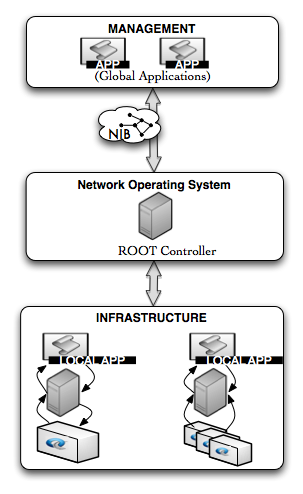
\includegraphics[scale =0.7]{pic/related/kandoo-design}
  \caption[Kandoo design] {Kandoo decomposes the control plane into 
in two levels. The root controller and global applications have access to the global network sate.  The Local controller and applications remain close to the data plane and do not require access to the global state.} 
  \label{fig:kandoo-design}
\end{figure}

%relief 
%The major goal is to shield the root controller from frequent events that could be processed without much knowledge of the network state.
%This two level design allows  shielding the controller from frequent events triggered by the network devices. 


%In Kandoo scalability is supported by the introduction of the two level hierarchy. 
%The bottom control plane  shields the root control from processing of events. 

We conclude with two points. 
First, the Kandoo architecture is complementary to others (even ours). 
%In fact the authors' stress that other distributed control planes and Kandoo can co-exist together. 
Second, Kandoo can effectively scale the control plane further at least in theory. 
However, Kandoo architecture is only as effective as the number of flows that it can process locally. 
%the effectiveness of scalability mechanism depends on a significant number of applications that are able to process flow requests locally without the root controller intervention. 
Unfortunely, the paper does not specifies how practical or significant are  the class of applications that can operate without global state as to process events locally. 

\subsection{HyperFlow}
\label{sec:related:hyperflow}



Motivated by the lack of scalability in centralized controllers, HyperFlow \cite{Tootoonchian:2010vy}  was created as a distributed controller. 
The  authors' aim was to provide scalability without sacrificing the simplicity of management applications  in centralized controllers. 
It is built as a \emph{C++} application on top of the NOX  controller \cite{Gude:2008jd} requiring minor modifications to the controller core and is not publicly available. 

Fig.~\ref{fig:hyperflow-design} shows the overall architecture of HyperFlow. 
The control plane is distributed over different controller instances (or replicas). 
Each instance maintains, under its administrative domain, the connection to a subset of the data plane. In case of failure, there should exist mechanisms that allow other controller to assume control of the failed controller data plane set. 

%Two main components compose this architecture: the controller application (HyperFlow) and an Publish/Subscribe middleware.  
%The controller component is an application, built in NOX, which interposes between NOX applications and the data plane to intercept all communication between the two. 
%To clarify, the controller intercepts event triggered by the data plane or applications as well as the configurations messages sent from the applications to the switches. 
%The controller component is an application built in NOX which intercepts events triggered by the data plane or the applications as well as the   configuration messages sent from the applications to the switches (i.e., commands). 
%In essence the controller interposes between NOX applications and the data plane capturing all communication between the two. 

In HyperFlow, each controller instance is a replica of the entire network state. 
To do so, HyperFlow intercepts any event that has caused changes to the network state (when processed by an application). 
Then, it distributes this event to other controllers that  will also process it. 
This way  --- and assuming that all controller instances run the same set of deterministic application --- all controllers instances eventually arrive at the same state.\footnote{Considering that there are no updates for a sufficient amount of time.}

The positive side in having a view of the entire network is that each controller can take decisions based on the state present locally.
%This state is eventually consistent since it will, at some point in time, be equal in all replicas\footnote{Considering that there are no updates for a sufficient amount of time.}. 
However, the controller still has to communicate with others to distribute state changing events and configuration directives to switches that are controlled by other instances. 


The inter-controller communication system is based on the well-known \emph{Publish/Subscribe} model, whereby one defines publishers as senders of messages and subscribers as the receivers. 
Publishers do not send messages directly  to receivers.  
Instead, messages are published in a medium, and interested receivers selectively receive them through some form of subscription logic (e.g., channel, topics, etc.). 
This model allows the decoupling of both space and time in the communication between publishers and subscribers. 

HyperFlow, leverages on an existing Publish/Subscribe system that provides: persistent storage of the events published; \emph{FIFO}
(First-In-First-Out)  ordered delivery of the messages published by the same controller; and resilience against network partitioning.
%The event propagation system allows  communication between HyperFlow instances and  is built over a distributed filesystem. 
%Communication is done through channels implemented as files. 
%There are three types of channels: the control channel where controllers advertise themselves; the data channel where general interest events are published by every controller;  and finally the individual controller channel for OpenFlow commands relevant to the controller who owns the channel. 

% State distribution in HyperFlow is accomplished through the
% Publish/Subscribe event propagation system. The NIB  is
% replicated in all instances and HyperFlow distributes the events
% that cause changes to it. This is done through event publishing in the shared
% data channel. Every controller subscribes to the
% data channel and replays the events received on it, thus changing its
% NIB in a similar way.  The view  is maintained by the Management applications
% residing in the controller and outside the domain of
% HyperFlow (as in NOX). HyperFlow is, in concept,  identical to a \gls{smr} system with the controllers as replicas. State changing events are distributed to all replicas, that execute them to converge to the same state of others. 


%Additionally, Hyperflow  also addresses incorrectness problems caused by transient inconsistency across controllers  by defining an \emph{authoritative}  controller for each flow. This controller is responsible for orchestrating changes in the network regarding some flow. As an example, to avoid loop-free forwarding \emph{authoritative} controllers are solely  responsible for setting the flow paths across the forwarding plane for some specific flow. For this, applications must relay requests for some flow to its \emph{authoritative} controller. 

HyperFlow addresses scalability of the control plane by minimizing the number of events that an instance replicates to others. 
Thus, HyperFlows s focus on the scalability of the CPU and does not address state scalability since  each controller contains  the entire network state. 

To minimize the number of events  processed by instances, HyperFlow filters the dissemination of events.  
To this end, it requires that applications tag locally generated events that affect the network state.   
Only these events are worth distributing,  as others are redundant. 


%Local events are generated either by the management or data plane layers but applications trigger events as a response to the processing of other events (i.e., there is a causality relationship between events). 
HyperFlow minimizes distribution of events even further by tracking events that cause other events. 
For this reason applications triggering events have to  associate the event that caused it. 
If, for example, some event $e_2$ is triggered due to the processing event $e_1$, it  distributes only event $e_1$. 
This is enough since the applications are equal in all controllers. 
Thus,  the processing of $e_1$ will  trigger event $e_2$ in all replicas. 
As one single event can cause several application events to be triggered this can reduce the volume of traffic and processing of redundant events.

\begin{figure}
  \centering 
  \footnotesize
  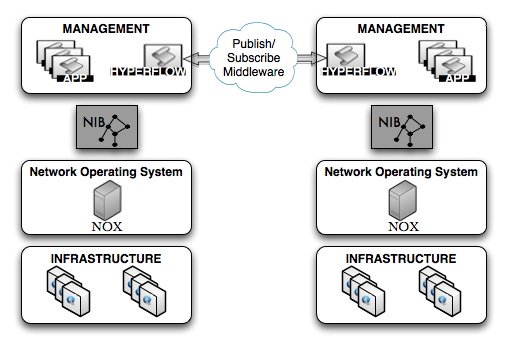
\includegraphics[width=\textwidth]{pic/related/hyperflow-design}
  \caption[HyperFlow architecture]{HyperFlow architecture. The two major components are the controller which intercepts events and configuration commands that must be distributed and the Publish/Subscribe system used for all communication between controllers.} 
  \label{fig:hyperflow-design}
\end{figure}

%Applications running on HyperFlow act as they control the entire network.
%Behind the scenes, HyperFlow redirects requests to the network equipment  to the controller equipment which the request addresses. 
%HyperFlow also routes back  responses to the controller responsible for  the request. 

One of the advantages of HyperFlow is that the existent applications are barely modified in order to work in a distributed control plane. 
Furthermore, the programming model itself is identical to NOX  (event driven, pipeline based) which maintains its simplicity and quite transparent since applications behave as they were running the all network. 
%Some overhead complexity is added as HyperFlow requires the applications to tag  state changing events and identify parent events as explained above. 

However, this is not quite true since applications do have to account for the restrictions of the underlying distribution system. 
For example, applications are limited to change state based only in events that arrive from a single switch. 
A complex Load balancer that wishes to perform aggregation calculations on more that one link across different switches would possibly result in divergent state across controller replicas. 
Notice that even with FIFO based channels some controller $c$ might receive event $e_i$ followed by event $e_j$ sent from controllers $i$ and $j$, while a controller $c'$ perceives $e_j$ followed by $e_i$. 
Thus, It is possible that such occurrence leads controllers to divergent states if applications modify state relying in event ordering across different entities. 
%For this not to happen each switch associated state could as well be completely isolated from
%The article explicitly adverts that Management applications should not rely in event ordering "except those targeting the same entity (e.g., the same switch or link)'' as those guarantee FIFO ordering. 

Another benefit of HyperFlow is that under read intensive workloads the controller can achieve low response times since  events are processed locally.
However in our experience with centralized applications (as the ones that HyperFlow targets) read intensive workloads are not too common.
In fact, Chapter~\ref{sec:feasibility:apps} shows that  three (out of three) applications in the Floodlight controller show at least one write operation for each event processed at the controller. 
We note that those applications are fundamental for tracking hosts, forwarding and round-robin load balancing and they could not easily  avoid that write operation without incurring in non-optimal behavior (i.e., they would be less correct in the goal they promise to achieve). 

%Finally, while HyperFlow is robust in the face of failure it does so at the expense of the controller resources. 
%Under failure it has to replay all events. This can be time consuming and events grow indefinitely. Under this time the controller can not serve requests. If instead this recovery mechanism is isolated from the controllers then a recovered controller (or other in its place) can start processing network events almost immediately. 
%Another benefit it that it requires minor modifications to a centralized controller. We note that this not exactly true. Given the restrictions imposed by the \gls{fifo} semantics of the publish subscribe middleware, the applications are not able to rely not even on causality modifications to the network state. An Load Balancer application that typically relies on different switch state to manipulate 


\subsection{Onix}
\label{sec:related:onix}

Onix \cite{Koponen:2010th}  was build upon the NOX legacy and provides two major contributions: it is the first general controller published in the literature, and also the first to provide strong consistency.  
Onix  provides an improved Network Operating System interface on  which the northbound API does not reflect the southbound API. 
Management applications are programmed against a network graph of Typed Entities very similar to the Object Oriented paradigm and are not aware of the southbound characteristics (e.g., the use of \gls{of}). 
The graph is implemented in  the \gls{nib}  --- a in-memory data structure that contains the network state ---  and can be distributed across a  cluster of  Onix controllers. 
Applications have the choice to specify consistency and durability requirements  per network entity  present in the \gls{nib}.  
Onix was the result of a joint effort between Google, NEC, Nicira, ISCI and Berkely, and (at least)  both Google and Ericson have developed their controllers based on from Onix \cite{The-Valley-of-the-Nerd.:fk}. 
At the time of writing Onix is not publicly available. 

Onix architecture is presented in figure \ref{fig:onix-design}. 
Only one application resides on the  Management layer and may communicate with other applications in other controllers instances for coordination. 
The \gls{nib} is the only element in Onix northbound interface. 
The Management layer directly modifies the \gls{nib} and subscribes to changes on it. 
The data plane  indirectly modifies the \gls{nib} (trough the controller).


The controller  has to guarantee that changes in the Infrastructure are reflected in the \gls{nib} and vice versa. 
For this, it translates network events into changes in the \gls{nib} and changes in the \gls{nib} to changes in the data plane configuration. 
Onix supports  \gls{of} but it could transparently move to another southbound API. 

Each Onix instance independently manages a subset of the data plane. 
However each instance can be exposed to the entire network state through  the \gls{nib}.  
Under such scenario, each time a local Onix instance alters the \gls{nib}, these changes are reflected in all other instances. 
Thus, the \gls{nib} is also the distribution mechanism of the Onix controller. 
The distribution itself is done by the datastores that back up  the \gls{nib} state (seen in figure \ref{fig:onix-design}).
However, in concept the \gls{nib} is not meant to contain all the network state. 
In fact, the \gls{nib} is best seen as a kind of in-memory cache which imports (exports) particular state from  (to) the fault-tolerant distributed data stores. 

\begin{figure}
  \centering 
  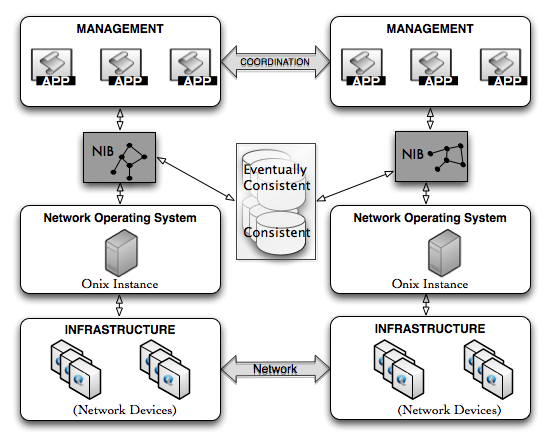
\includegraphics[width=\textwidth]{pic/related/onix-design}
  \caption[Onix architecture] {\textbf{Onix achitecture.} In Onix the NIB is the
    solely entity used as the northbound api and Managements program
    directly against it. The NIB is supported by
    two replicated datastores accessible across Onix instances.  The
    Management layer communicates across instances for coordination.}
  \label{fig:onix-design}
\end{figure}

% \begin{figure}
%   \centering 
%   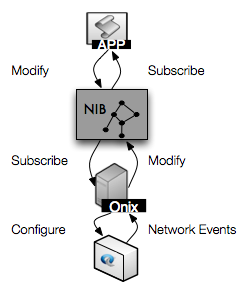
\includegraphics[scale=0.5]{pic/onix-process.png}
%   \caption[Onix configuration process]{\textbf{Onix configuration
%       process}. The interactions between layers of the Onix
%     instance stack. In the figure we can observe the process of
%     configuration on the left side, and the process of detecting
%     changes in the Infrastructure on the right side.\footnote{The Infrastructure should be only one.}} 
%   \label{fig:onix-process}
% \end{figure}

Onix defines a flexible distribution model for the \gls{nib} whereby  it offers the application designer the choice of consistency guarantees. 
Two replicated data stores are present, covering  strong  and eventually consistency. 
Strong consistency data is provided through a transactional persistent database backed up by a replicated state machine (see section~\ref{sec:related:cons-data-stor}). 
This data store is favored for data with low-frequency changes  as its performance limitations are significant. 
The eventually consistent data store consists in  an one hop memory based \gls{dht}  (as Dynamo  \cite{DeCandia:2007cn}) favored for  volatile data with high update rates. 
%The \gls{nib} reflects the state of both data stores. 
Both the integration of multiple data stores and the inconsistency characteristics of the \gls{dht} can lead the \gls{nib} to an inconsistent state where reads performed in some entity may return more than one result. 
Thus, Onix provides primitives for the integration of inconsistency resolution logic as well as  direct integration of a distributed coordination framework (see  Apache' ZooKeeper \cite{Hunt:2010ux}) in the northbound interface. 

Onix is intended for large scale network infrastructure where scalability is fundamental. 
However, in each Onix instance the \gls{nib}  size reflecting the network state could lead to memory exhaustion and the processing of both network events and subscriptions  to changes in  the \gls{nib}  can lead to \gls{cpu} exhaustion.
In order to introduce scalability and avoid exhaustion, partition and aggregation based techniques can be configured in the Management layer. 
Partition avoids full replication of both data  and workload such that additional instances do not only replicate overall work but also relief it. 
As for aggregation it can, for example, allow network entities to be aggregated and exposed for other Onix instances as only one.
In practice partition in Onix is present in the division of the data plane across different Onix instances.  
This way instances process fewer events. 
Additionally the Management logic can configure Onix instances to keep only subsets of the \gls{nib} in memory and up to date. 
For aggregation, an Onix instance can be configured to expose a subset of the \gls{nib} as an aggregated element. 
%MISSING THINGS . To exemplify a controller could export, to the data stores, its network topology as a single 

Applications are built against the \gls{nib} graph data structure that is composed of \emph{Typed Entities} supporting the Object Oriented paradigm (i.e., encapsulation of data, functions over entities, hierarchy, etc.). 
Onix supports extensible representations of network entities. 
The \gls{api}  provides essential functions to search, inspect, create, destroy and modify entities present in the \gls{nib}. 
It is also possible to register notifications for creation, removal and updates of data entities. 
When network events of other Onix instances update the data stores those changes must be reflected on the local \gls{nib} and the application must be notified through a callback function. 
All operations are asynchronous, with eventual delivery and no ordering or latency guarantees given therefore a \emph{barrier} synchronization primitive is available allowing the application to wait as updates are translated and applied in the network devices and/or other controllers. 
Finally it is worth mentioning that Onix employs coarse-grained locking mechanisms over the \gls{nib}.
 Applications are given the guarantee that no other local thread concurrently updates the \gls{nib}. 


Onix is focused in generality; and it does a great job at it. 
However it is merely an control platform where the Management application has to fill-in to complete  most of the work. 
Namely, neither reliability nor scalability are first class citizens of the platform. 
Furthermore, beyond delegating reliability for the developer, Onix relies on third party applications for this task (i.e., Apache' Zookeeper~\cite{Hun10} ). 
This, it introduces another degree of complexity for the \gls{sdn} developer which has to learn yet another interface. 
As a contrast, in our controller design the same interface is able to perform all the tasks which (arguably) presents a less steeper learning curve.  

It is important to realize that Onix is in no way optimized for performance. 
As stated in the paper: ``when faced with a tradeoff between generality and control plane performance we try to optimize the former while satisfying the latter''. 
This is fine, but it lefts us (the world) with a gap in the research field. 
Namely we need to understand what kind of impact does a reliable and distributed control plane has on real world \gls{sdn} applications. 
Furthermore, we need to effectively contrast eventual consistency vs. strong consistency distributed control planes. 
To clarify, not even the Onix eventual consistent  data store evaluation is able to show a significant performance advantage against an off-the-shelf consistent data store.  
This is bad, since enterprises currently, have no way to accurately determine, based on the number of events generated by their data planes, what kind of consistency semantics they should seek for their distributed \gls{sdn} deployment. 

Finally we note that Onix is all but transparent. 
Applications have to include conflict resolution logic, and rely on different interfaces for the appropriate semantic per action. 
To clarify, applications must choose between eventual consistency, strong consistency, à priori in a statically defined import/export module. 
Furthermore, they must rely on complex event oriented programming techniques and specific \gls{nib} methods as the barrier primitive or external interfaces as Apache Zookeeper to modify state with a coherent and reliable semantics. 

%%%%%%%%%%%%%%%%%%%%%%%%%%%%%%%%%%%%%%%%%%%%%%%%%%
\glsresetall
\section{Consistent Data Stores}
\label{sec:related:cons-data-stor}

The key idea of our controller architecture is to make the controller instances coordinate their actions through a dependable data store in which all relevant state of the network and of its control applications is maintained in a consistent way.
This data store is implemented with a set of servers (replicas) to avoid any single point of failure, without impairing consistency.
One of the most popular techniques for implementing such replicated data store is \gls{smr}~\cite{Schneider:1990vy,Lam98}.

The  \gls{smr} technique provides one of the most strongest consistency model known in distributed systems named linearizability. 
This model is completely transparent for the client of the system; so transparent that it is indistinguishable from a centralized (i.e., non-replicated) system. 
Off course, this is at the expense of performance, and more importantly availability since in order to operate it requires a majority of the systems replicas to be accessible. 
The remaining spectrum of consistency models is under the umbrella of the eventual consistency semantics. 
%This model is somewhat undefined, and can support quite mean different  
With eventual consistent data stores, data is also replicated in different replicas. 
However, several problems can emerge from this model including (but not limited) the loss of updates and  conflicting values. 
We give a detailed description and examples of both consistency models in section~\ref{sec:related:underst-cons}.

Practical crash fault-tolerant replicated state machines are usually based on the Paxos agreement algorithm for ensuring that all updates to the data store are applied in the same order in all replicas (thus ensuring consistency)~\cite{Lam98}. 

However, since the original Paxos describes only an algorithmic framework for maintaining synchronized replicas with minimal assumptions, we instead describe --- in section~\ref{sec:related:viewst-repl} ---- the Viewstamped Replication (VR) protocol, a similar (but more concrete) state machine replication algorithm introduced at the same time~\cite{,Liskov:2012ut}\footnote{Also, the Paxos algorithm is known for being hard to understand.}.


State Machine Replication is a fundamental technique that is used by real world systems in a wide array of applications. Furthermore, and contrary to popular believe, it can be used in systems where  availability and performance are crucial requirements.  As so, in section~\ref{sec:related:state-mach-repl} we give an overview of state of the art performance of \gls{smr} based systems. 


\subsection{Eventual Consistency}
\label{sec:related:underst-cons}

To understand consistency we must first establish some fundamental concepts. 
In our context the consistency discussion and tradeoffs arises from data replication systems such as data stores. 
Those systems are replicated for reliability and/or performance. 
The reliability benefit arises from the fact that failures are often the rule and not the exception. Therefore, data must be replicated across different servers in order to survive the time challenge. 
As for the performance benefit in can be manifested in two different forms. First, different replicas can be located closer to different clients therefore improving on the latency. Second, client load can be balanced across different replicas therefore improving the limit on the system processing rate. 


Since the proof of the CAP theorem in 2002 by Gilbert and Lynch that there is an significant  interest in weak consistent distributed systems~\cite{Gilbert:2002il}. 
This theorem establishes that a distributed system can only be qualified with only two of the following properties: consistency, availability and partition-tolerance. 
In this context, consistency is equivalent to a system supporting linearizability (which will be defined in a moment), availability is equivalent to the guarantee than any request performed on the system eventually receives an reply, and partition-tolerance implies  tolerating arbitrary message loss. 
Being that systems  often exhibit arbitrary message loss caused by the network or other pitfalls (the nodes might be  stuck processing the garbage collector algorithm) systems are force to choose between availability and consistency. 

Facing those facts a replicated system is either consistent or eventually consistent. 
If consistent than it is not always available; if eventually consistent it is always available. 
But in practice systems are not black or white. 
In fact, one of the outcomes of the dichotomy established by CAP is a panoply of systems with different consistency models that attempt to position themselves at a different optimal point between  the availability and consistency spectrum. 
To explain, if we look under the hood of eventually consistent, we will conclude that  this model is an umbrella for different consistency models that can be ``more or less'' consistent (e.g., read-your-writes, causal consistency, session consistency). 
Due to space constraints we cannot cover each of those models and instead defer the interested reader for surveys on the topic \cite{bailis2013eventual, bailis2013eventual}

%For simplicity we will focus on the contrast between eventual and strong consistency. 

%To simplify the discussion let us imagine that each client can only issue a single write operation. 


Under the \textbf{eventual consistency} model when a write is finished, then the model promises that at some point in time all clients will converge to the same value. 
The benefit with those models is that they are straightfoward to implement. 
A replica can accept client requests, process them, return the result and only later spread the outcome to others. 
The process of spreading values to others is commonly known as anti-entropy and can take several forms but it in essence an asynchronous (i.e., after replying to the client) process. 
Therefore, several ``bad'' outcomes can come out of it. 
We will show three. 

For support, let us imagine a replicated system with three replicas and only a single register containing some arbitrary value. There are two clients of the system: client 1 and 2 that can perform write and read operations on this register. Fig.~\ref{fig:related:eventual} shows the system composition with two examples of different client requests orderings. 

\begin{figure}
  \centering
  \begin{subfigure}[b]{0.5\textwidth}
                \centering
                \includegraphics[width=\textwidth]{pic/related/eventual-conflict}
                \caption{Stale data: reading an old value.}
                \label{fig:related:eventual-stale}
        \end{subfigure}%
        ~
        \begin{subfigure}[b]{0.5\textwidth}
                \centering
                \includegraphics[width=\textwidth]{pic/related/eventual-stale}
                \caption{Conflicting data.}
                \label{fig:related:eventual-conflict}
        \end{subfigure}
  \caption[Eventual Consistency pitfalls]{Two clients of a replicated data store experiencing some of the eventual consistency model pitfalls. In the stale data case Client 2 is not able to see the last write done to the data store. As for the conflicting data case the concurrent update done  by two clients causes the data store to become confused as to what value it should keep.}
\label{fig:related:eventual}
\end{figure}


First,  Fig.~\ref{fig:related:eventual-stale} shows than while replicas have not converge on client updates other clients are able to see older values of the register. 
Namely, client 1 performs an update on the data store ($write(x)$) and after an certain amout time client 2 stills sees the older value of the register ($Y$). 
We note that with weak eventual consistency models not even Client 1 could be assured to read X in a follow up operation. 
This particular safety property is known as read-your-writes consistency and commonly requires that clients contact with the same replica of the system\footnote{Off course this is only the case for eventually consistency systems. Strong consistency does not imposes this restrictions abeit offering read-your-writes guarantee.}. 
The time period between a write being applied in a data store replica and all clients being able to see that value is named the \textbf{window of inconsistency}.  A position paper on eventually consistent systems states that this window of inconsistency is bound between 200 ms to 15 seconds in different types of systems\cite{bailis2013eventual}. Due to the differences in the environment where those tests were performed we show those values as reference to show that state of the art eventually consistent data stores maintain a lower bound of 200 ms. 

It might be the case that the bound on the  window of inconsistency is not problematic for the users of the  data store. 
However a subtle problem can emerge from the asynhronous anti-entropy process ---- there is no guarantee that an update will reach other clients. 
This it to say that when gets a reply from a server to an update operation (e.g., $write(x)$)  he can not be sure that this update will eventually be seen at other clients. 
First, it might be the case that concurrent updates from other clients cause the loss of the update. 
Surely this is also the case for consistent data stores, but it also true that it is much harder to contradict this behaviour in eventual consistent systems than in strong consistent systems (to see an example of this see section~\ref{sec:heimdall:versioning}). 
Second, and arguably more serious problem than the one identified in the previous argument, it might be case that the server that processed the update fails before spreading it to other replicas. 
In the event that this happens, it can also be the case that recovery is not supported by the system which ineviatably leads to updates being lost forever. 
Thefore, eventually consistency ensures convergence only if replicas survive long enough do spread updates to others. 


Finally, in the event of concurrent updates to a particular data bucket (e.g., our register) eventually consistent systems are forced to deal with conflicting values. 
Fig.~\ref{fig:related:eventual-conflict} exemplifies that  both clients concurrently update the register. 
Then, imagine that two different data store replicas (out of three) process and reply to the clients independently. 
Later on, the anti-entropy process takes place. The question that must be answered then is the following: how out the replicas be able to determine which update should persist between the two ($write(X), write(Y)$). 
Surely only one can be choosen, and undoubtely in many cases it should be lastest. 
However without heavy-weight premises and abstractions  such as the ones used in real-time systems it becomes impossible to determine which update was the lastest. 
Furthermore, it might be the case that the client 1 write is more important than client 2. 
Eventually consistent systems diverge in how they arbiter conflicts. 
Commonly either the system solves the conflict automatically without user intervection, or both values are kept and the uses out to solve this. 
Given that from the system point of view data is just an opaque arbitrary collection of bytes (i.e., raw data) , it is forced to crude arbitration such ``last-write-wins'' (which is commonly not based on a global wall-clock time). It is also the case that more sophisticated systems have a more deep understanding of their data. 
For example, the use of a \gls{crdt} such as a set allows the data store to follow a simple conflict resolution policy  based on a simple union of all the conflicting sets~\cite{shapiro:inria-00555588}. 
On the other hand, delegating conflict resolution to the clients leverages the benefit that the latter is well-aware of the data schema present in the data store as well as the semantical meaning of the two conflicting values. 
As such it can be better equipped to choose how to solve conflicting values.
Notwithstanding  the evidence that systems are equipped to deal with conflicts they do so at the expense of possible incorrectness (in the system case) or the extra effort required from the developer that has to anticipate conflict resolution code for different types of data. 

%Two different approaches can be taken: the system can choose one of the conflicting values and discard all the others; the system can keep both and the 
%In contrast, with the strong consistency model users are not able to discover that data is replicated. 
%In fact the client of systems that provide this model are not able to distinguish him in any way from a centralized system. 

In general, eventually consistent data stores are better equipped to deal with volatile data that does not have stringent requirements such as consistency and reliability.
With the lack of consistency clients are not able to reliable  synchronize with others nor can anticipate the results of an update. 
To combat this lack of guarantees clients must develop counter-measures when dealing with more sensible data that can not rely on the pitfalls seen in this section. 
This implies that additional effort and time must be taken from developers being that in the end they are still subjected to corner cases that they were not able to anticipate  that could arguably result in the failure of the overall system. 

%In opposition the use of strong consistency 
%The users of an eventual consistency are not CONDENADOS to all this pitfalls. However as stated by Bailis et. al, the user has to ``compensate'' for the lack of consistency.  There are techniques that avoid this A \gls{crdt} CRDt's Although these are prominent research topics, these are still concepts difficult to master to the regular developers.

\subsection{Strong Consistency}
As Fekete and Ramamrithan so eloquently state : ``the principal goal of research on consistency models is to help application developers understand the behavior they will see when they interact with a replicated storage system, and especially so they can choose application logic that will unction sensibly''. \cite{fekete2010consistency}
Indeed, for the user a properly defined semantics associated with the requests performed on replicated systems is of paramount important. 
Without it, the user might be able to commit ``mistakes'' that sacrifice the reliability of the data. 
In this context, the most significant advantage of the strong consistency model  is that developers can relax their concern towards the semantics of the replicated system being that a strong consistent system is not any different from a centralized (single site), unreplicated system --- there is no more transparent system that this. 

Truly, the strong consistency property is formally introduced as linearizability~\cite{herlihy1990linearizability} in a seminal paper by Herlihy~\etal. 
In the paper the reader may find a formal definition of linearizability. 
Informally, this property establishes that every operation performed on the replicated systems appears to have effect instantaneously. 
The practical consequence is that clients can be made sure that after receiving a reply from the system for an update operation every other client will be able to see the effect of that write. In practice, this condition is true as soon as the data store processes the client update, but it makes more sense, from the client point of view, to base this assumption only as soon as the reply arrives since it has no other mean to determine that the data store has processed his operation. Fig.~\ref{fig:related:strong} exemplifies this condition. 

Strong consistency is great, since clients are now able to accurate rely on the data store reliability property as soon as they receive a reply. 
To exemplify, the \gls{smr} technique that we use (covered in the following section) blocks client requests until they are processed by a majority of replicas that compose the system. 
Given that this techniques assumes that there will always be a majority of replicas ``alive'' (i.e., non faulty) and reachable, the client is made sure that the aforementioned operation will never be lost in the data store unless it is overwritten. 
However, using simple concurrency control techniques (see section~\ref{sec:heimdall:versioning}) clients can also be sure that no client will innocently overwrite its data without at least  be made aware of it. 
If clients behave correctly they can always confirm in the data store that they are aware of the least-recently-update thus avoiding overwriting data.

\begin{figure}
  \centering
  \includegraphics[width=0.5\textwidth]{pic/related/strong-consistency}
  \caption[Strong Consistency Semantics]{Strong Consistency Semantics. A client can be sure that every client see its operation outcome as soon as the data store replies.}
  \label{fig:related:strong}
\end{figure}
Strong consistent or linearizable distributed systems enable coordination between distributed applications. 
Coordination is a complex problem. For this reason it is desirable to solve once in a generic fashion such that different applications can make benefit from its application. 
A common example of coordination use cases is group membership and leader election.
It is often the case than distributed nodes need to known which nodes are alive and partition responsibility amongst them. 
There are several applications inspired by those particular problems such as Apache' Zookeeper~\cite{Hun10} and Chubby~\cite{burrows2006chubby}. 
And at the very heart of it relies protocols that guarantee strong consistency in distributed replicated systems. 

\subsection{ViewStamped Replication}
\label{sec:related:viewst-repl}
\glsreset{smr} 
The Viewstamped (VR) protocol provides a transparent \gls{smr}  behavior that can be leveraged to implement a replicated data store with strong consistency semantics~\cite{Liskov:2012ut,Liskov:2010vt}. 
The algorithm is built over  an partial-asynchronous network model with a crash-recover failure model for the participants (\emph{replicas}) who are the basis for maintaining a data service  available to clients. 

\gls{smr} allows a set of machines to provide a replicated service, usually to support  availability and reliability characteristics in the system~\cite{Schneider:1990vy}.  
Informally,  the model states that a distinguished set of machines who start in the same state and execute the same set of instructions in the same order achieve the same state  and generate the same output. 
\gls{smr} is suitable for  distributed applications, such as  file systems or lock managers which can  be built on top of the distributed state machine. 

The failure and timing model establishes that replicas may stop (due to crash), perform computations arbitrarily slow or  be isolated from the rest of the group. 
The remanning  group detects and suspects the replica has failed as a reaction to its lack of feedback.
VR allows replicas to re-join the group as long as they are updated on the missed executions by the other replicas.
VR  runs in a Replica Group composed of at least $2f+1$ replicas and assumes that only $f$ replicas can fail simultaneously. 
Thus, as long as $f+1$ replicas are accessible the protocol guarantees liveness (which translates to availability from the client point of view). 

\begin{figure}
\centering
\includegraphics[width=\textwidth]{pic/related/vr.pdf}
\caption[Paxos/VR update protocol]{Paxos/VR update protocol.} 
\label{fig:paxos} 
\end{figure}

VR is based on  \emph{total-order}, a ordered delivery guarantee between a set of machines communicating in group. 
The protocol has a behavior structured around the notion of a leader (a distinguished replica named primary) who chooses and imposes the order of delivery of executions on the group. 
This approach has the drawback of overloading the primary with client requests but  simplifies the protocol and reduces execution latency significantly. 


Fig. \ref{fig:paxos} shows the messages exchanged in VR for an update operation: the client sends a message to a primary replica (the leader) that disseminates the update to all other replicas. 
These replicas write the update to their log and send an \texttt{ACK} message to the primary.
In the final step the leader executes the request and sends the reply to the client.
If the primary fails, messages will not be ordered and thus a new primary will be elected to ensure the algorithm makes progress.
When read-only operations are invoked, the leader can answer them without contacting the other replicas.
Strong consistency is ensured due to the fact that all requests are serialized by the leader.

Off course this is only the normal execution of the protocol. 
The interest reader is forwarded to the originals papers  for a description of the remaining protocol which involves a protocol for re-electing a new leader of the system whenever the current is suspected to fail and also a protocol for recovering replicas such that they can be updated by the group~\cite{Liskov:2012ut,Liskov:2010vt}. 
%Each replica runs the same application code as each can be the primary at some point in time.



\subsection{State Machine Replication Performance}
\label{sec:related:state-mach-repl}
The Paxos/VR algorithm has served as the foundation for many recent replicated (consistent and fault-tolerant) data stores, from main-memory databases with the purpose of implementing coordination and configuration management (e.g., Apache'  Zookeeper~\cite{Hun10}), to experimental block-based data stores or virtual discs~\cite{Rao11,Bol11,Bes13}, and even to wide-area replication systems, such as Google Spanner~\cite{Corbett:2012uz}.
Besides the synchronization protocol, these systems employ many implementation techniques to efficiently use the network and storage media.

Although not as scalable as a weakly consistent data store, these systems grant the advantages of consistency for a large number of applications, namely those with moderate performance and scalability requirements. To give an idea of the performance of these systems, Table \ref{table:smr-results} shows the reported throughput for read and write operations of several state-of-the-art consistent data stores.

\begin{table}
  \center
    \begin{tabular}{ lccc}
    \hline
    \emph{System} & \emph{Block Size} & \emph{kRead/s} & \emph{kWrite/s} \\ \toprule
    Spanner \cite{Corbett:2012uz} & 4kB & 11 & 4 \\ 
    Spinnaker \cite{Rao11} & 4kB & 45+ & 4 \\  
    SCKV-Store \cite{Bes13} & 4kB & N/R & 4.7 \\ 
    Zookeeper \cite{Hun10} & 1kB & 87 & 21 \\ \bottomrule 
    \end{tabular}
  \caption[Performance of state machine replication systems]{Throughput (in thousands data block reads and writes per second) of consistent and fault-tolerant data stores based on state machine replication (N/R = Not Reported).}
  \label{table:smr-results}
\end{table}

Given the differences in the design and the environments where these measurements were taken, we present these values here only as supporting arguments for the possibility of using consistent data stores for storing the relevant state of SDN control applications.
Depending on the specific application this state may include, for instance, a subset of the Network Information Base (NIB).
Interestingly, these values are of the same order of magnitude of the reported values for \emph{non-consistent} updates in Onix (33k small updates per second considering 3 nodes~\cite{Koponen:2010th}), and much higher than the reported values for their consistent data store (50 updates/second for transactions with a single update).
The Onix paper does not describe how its consistent database is implemented but, as shown by these results, its performance is far from what is being reported in the current literature.

%%%%%%%%%%%%%%%%%%%%%%%%%%%%%%%%%%%%%%%%%%%%%%%%%%
\glsresetall
\section{Consistent Data Planes}
\label{sec:related:consistent-data-plane}


\subsection{Consistent Updates}
The authors' recognize that networks are in constant change. 
Routing policy, access control for severals reasons. 
Updates can disrupt the network. 

%%% Local Variables: 
%%% mode: latex
%%% TeX-master: "../PEI"
%%% End: 
